\chapter{Software portability}\label{porting}

Ideally, any software would be usable on any operating system, platform, and any processor architecture.
Existence of term "porting", derived from the Latin portāre which means "to~carry", proves that this ideal situation does not occurs that often, and the actual process of "carrying" software to a system with a different environment is often required.
Porting is process required to adapt software designed for specific platform to another platform.
Porting is also used to describe process of converting computer games to become platform independent\cite{wiki_porting}.

Software porting process might be hard to distinguish from building software.
The reason might be that in many cases, re-building software on the desired platform is enough.

Nowadays, the goal should be to develop software which is portable between preferred computer platforms (Linux, UNIX, Apple, Microsoft).
If the software is considered as not portable, it does not have to mean that it is not possible, just that the time and resources spent porting already written software are almost comparable, or even significantly higher than writing software as a whole from scratch.
Effort spent porting some software product to work on a desired platform must be little, such as copying already installed files from one computer to another and run/re-build it.
This kind of approach might most probably fail, due to not present dependencies of third party libraries on the destination computer.
Despite dominance of the x86 architecture, there is usually a need to recompile software running, not only on different operating systems, to make sure we have all the dependencies present.

Number of significantly different central processor units (CPUs), and operating systems used on the desktop or the server is much smaller than in the past.
However, on embedded devices market, there are still much more various architectures available including ARM\footnote{https://www.arm.com/products/processors} or MIPS\footnote{https://www.mips.com/products/classic/}.

To simplify portability, even on processors with distant instruction sets, modern compilers translate source code to a machine-independent intermediate code.
But still, in the embedded system market, where OpenWrt operating system belongs to, porting remains a significant issue \cite{porting_software}.



\section{OpenWrt System}\label{owrt}
OpenWrt is Linux distribution for embedded devices especially for wireless routers.
It was originally developed in January 2004 for the Linksys WRT54G with buildroot from the uClibc project.
Now it supports many more models of routers.
OpenWrt is a registered trademark which is held by the Software in the Public Interest (SPI) in the name of the OpenWrt project.

Installing OpenWrt system means replacing our router’s built-in firmware with the Linux system which provides a fully writable filesystem with package management.
This means that we are not bound to applications provided by the vendor.
A router (the embedded device) with this distribution can be used for anything that an embedded Linux system can be used for, from using its SSH Server for SSH Tunneling, to running lightweight server software (e.g. IRC server) on it.
In fact, it allows us to customize the device through the use of packages to suit any application. \cite{openwrt}



\subsection{OpenWrt and LEDE}

The LEDE Project (“Linux Embedded Development Environment”) is a Linux operating system emerged from the OpenWrt project.
Its announcement was sent on 3th May 2016 by Jo-Philipp Wich to both the OpenWrt development list and the new LEDE development list\footnote{https://lwn.net/Articles/686180/}.
It describes LEDE as "a reboot of the OpenWrt community" and as "a spin-off of the OpenWrt project" seeking to create an embedded-Linux development community "with a strong focus on transparency, collaboration and decentralisation"\footnote{https://www.phoronix.com/scan.php?page=news\_item\&px=OpenWRT-Forked-As-LEDE}.

The rationale given for the reboot was that OpenWrt suffered from longstanding issues that could not be fixed from within—namely, regarding internal processes and policies.
For instance, the announcement said, the number of developers is at an all-time low, but there is no process for on-boarding new developers and no process for granting commit access to new developers.

At the moment, the latest release of OpenWrt is 15.05.1 (code-named "Chaos Calmer") released in March 2016.
LEDE developers continued to work separately on their upstream release and they delivered LEDE "Reboot" with version 17.01.0 on February 22nd 2017.

The remerge proposal vote was passed by LEDE developers in June 2017\footnote{http://lists.infradead.org/pipermail/lede-adm/2017-June/000552.html}.
After long and sometimes slowly moving discussions about the specifics of the re-merge, with multiple similar proposals but little subsequent action, projects formally announced on LEDE forum in January 2018\footnote{https://forum.lede-project.org/t/announcing-the-openwrt-lede-merge/10217}.
OpenWrt and LEDE projects agreed upon their unification under the OpenWrt name.
After merge, OpenWrt upstream repository started to show signs of life.

Today (April 2018) the stable LEDE 17.01.4 "Reboot" release of OpenWrt released in October 2017 using Linux kernel version 4.4.92 runs on many routers \cite{lede_release}.



\subsection{Why Use OpenWrt}

Custom router firmware may be more stable than our hardware’s default firmware from the vendor.
Not even that, but probably more secure with regular security updates.
Besides OpenWrt, there is another open source Linux based firmware available such as Tomato or DD-WRT.

In the past OpenWrt has supported only CLI (command line interface) configuration, therefore, it was best match for software developers, network admins, or advanced users.
A user not acquainted with Linux or even not comfortable with CLI may find the OpenWrt platform hard to use and may turn to other available solutions.

The Tomato firmware is the best match for unexperienced users providing rich GUI and many other features, specifically live "visual" traffic monitoring, allowing easy visibility on inbound/outbound traffic in real-time.
Big disadvantage of the Tomato is that the list of supported devices is quite poor.

DD-WRT on the other hand, is compatible with more routers than any other third party firmware.
Compared to Tomato, DD-WRT is reported to have more bugs and less intuitive GUI.
The DD-WRT was known as the most feature rich firmware until OpenWrt came along.

OpenWrt turns our router in a fully capable GNU/Linux computer, not just a network "magic" box.
Recently, the OpenWrt platform has come a long way in making itself more accessible to all user levels.
It has an Luci\footnote{https://github.com/openwrt/luci} Web UI(user interface) now.
Users that are less experienced with Linux can easily set up their network using Luci.
OpenWrt is capable of running lightweight services like an IRC bouncer or samba/ftp file sharing (some routers have USB ports able to power HDD) or even run software build on our own\cite{vpnpick}.

The goal of this thesis would be to port a lightweight Tang daemon, described in the section \ref{tang}, to OpenWrt system.
Tang server will help us unlock our encrypted volumes while on safe home or office network without a need for extra PC running it but having it on our tiny OpenWrt "server".
With Tang, we do not have to care about typing passphrases over and over to unlock LUKS drives in a safe environment.



\section{OpenWrt's Tool-chain}

Compilation is done by set of tools called tool-chain and it consists of:
\begin{itemize}
    \item compiler
    \item linker
    \item a C standard library
\end{itemize}

Embedded devices are not meant for building on them because they do not have enough memory nor computation resources as ordinary personal computers do.
For example device specification see Table \ref{routerspec}.
Building on such device would be time consuming and may result in overheating, which could cause the hardware to fail.
For this particular reason, package building is done with cross-compiler.

Cross-compiler is a programming tool capable of creating an executable file that is supposed to run on a "target" architecture, in a similar or completely different environment, while working on a different "host" architecture.
It can also create object files used by linker.
The reason for using cross-compiling might be to separate the build environment from the target environment as well.
OpenWrt tool-chain uses gcc compiler, and it is one of the most important parts of tool-chain.

Most common C standard libraries are: GNU Libc, uClibc musl-libc, or dietlibc.
They provide macros, type definitions and functions for tasks such as input/output processing (<stdio.h>), memory management (<stdlib.h>), string handling (<string.h>), mathematical computations (<math.h>), and many more\footnote{https://en.wikipedia.org/wiki/C\_standard\_library\#Header\_files}.
The OpenWrt's cross-compilation tool-chain uses musl-libc.

For porting to "target" system (OpenWrt) this tool-chain has to be generated on "host" system.
The tool-chain can be created in many different ways.
The easiest way is undoubtedly to find a .rpm (.deb or any distribution specific package available) package and have it installed on our "host" system.
If a binary package with desired tool-chain is not available for our system or is not available at all, there might be a need to compile a custom tool-chain from scratch\footnote{tools like crosstool-ng (https://github.com/crosstool-ng/crosstool-ng) may help}.

In case of OpenWrt, we have an available set of Makefiles and patches called buildroot which is capable of generating tool-chain.



\section{OpenWrt's Buildroot}

OpenWrt's buildroot is a build system capable of generating the tool-chain, and also a root file-system (also called sysroot), an environment tightly bound to the target.
The build system can be configured for any device that is supported by OpenWrt.

The root file-system in general is a mere copy of the file system of target's platform.
In many cases, just having the folders /usr and /lib would be sufficient, therefore we do not need to copy nor create the entire target file system on our host.

It is a good idea to store all these things, the tool-chain and the root file-system in a single place.
With using OpenWrt's buildroot we will have this covered.
Be tidy and pedantic, because cross-compiling can easily become a painful mess!\cite{fabrizio}



\subsection{Buildroot Prerequisites}

Let us demonstrate minimum requirements of space and size of RAM for building packages for Openwrt using its buildroot.
For generating an installable OpenWrt firmware image file with a size of e.g. 8 MB, we will need at least:
\begin{itemize}
\item ca. 200 MB for OpenWrt build system
\item ca. 300 MB for OpenWrt build system with additional packages
\item ca. 2.1 GB for source packages downloaded during build from the Feeds
\item ca. 3-4 GB to build (i.e. cross-compile) OpenWrt and generate the firmware file
\item ca. 1-4 GB of RAM to build Openwrt
\end{itemize}

Table \ref{routerspec} lists the specifications of embedded device TL-WR842Nv3, a regular wireless router manufactured by TP-LINK, which was used to test all packages related to Tang server porting effort.

\begin{table}[H]
\centering
\label{routerspec}
\begin{tabular}{c|c}
\hline
Model           &   TL-WR842N(EU)                   \\ \hline
Version         &   v3                              \\ \hline
Architecture:   &   MIPS 24Kc                       \\ \hline
Manufacturer:   &   Qualcomm Atheros                \\ \hline
Bootloader:     &   U-Boot                          \\ \hline
System-On-Chip: &   Qualcomm Atheros QCA9531-BL3A   \\ \hline
CPU Speed:      &   650 MHz                         \\ \hline
Flash chip:     &   Winbond 25Q128CS16              \\ \hline
Flash size:     &   16 MiB                          \\ \hline
RAM chip:       &   Zentel A3R12E40CBF-8E           \\ \hline
RAM size:       &   64 MiB                          \\ \hline
Wireless:       &   Qualcomm Atheros QCA9531        \\ \hline
Antennae(s):    &   2 non-removable                 \\ \hline
Ethernet:       &   4 LAN, 1 WAN 10/100             \\ \hline
USB:            &   1 x 2.0                         \\ \hline
Serial:         &   No                              \\ \hline
\end{tabular}
\caption{TL-WR842Nv3 specifications}
\end{table}

Comparison of available storage space on wireless router to the actual sum of space required only for buildroot to work correctly, which is about 6.4 GB, should demonstrate why the building for embedded devices is done with cross-compiling.
Another reasons, not to just compare internal storage which might be extended\footnote{https://wiki.openwrt.org/doc/howto/extroot}, are device's minimalistic RAM size and low computation capability of the CPU.



\section{Preparing the Host Environment}

To start with cross-compilation on the host system, we need to set up an environment for it.
As the OpenWrt buildroot is a set of scripts, it has run-time dependencies.
We need to install these dependencies first.
To install buildroot dependencies on Fedora 27 system run:
\begin{lstlisting}[columns=fixed,basicstyle=\ttfamily\footnotesize,tabsize=4,backgroundcolor=\color{yellow!10}]
# dnf install binutils bzip2 gcc gcc-c++ \
    gawk gettext git-core flex ncurses-devel ncurses-compat-libs \
    zlib-devel zlib-static make patch perl-ExtUtils-MakeMaker \
    perl-Thread-Queue  glibc glibc-devel glibc-static quilt sed \
    sdcc intltool sharutils bison wget unzip openssl-devel
\end{lstlisting}
Some packages might be not available over git but only via other versioning tools like svn (subversion) or mercurial.
In our case this will not be necessary but if we want to obtain their source-code, we need to install svn and mercurial as well:
\begin{lstlisting}[columns=fixed,basicstyle=\ttfamily\footnotesize,tabsize=4,backgroundcolor=\color{yellow!10}]
# dnf install subversion mercurial
\end{lstlisting}
These commands have to be run by a user with root privileges.



\subsection{Getting Buildroot}

OpenWrt system has SDK (Software development kit) buildroots available for every released version of OpenWrt system.
It is good to consider using OpenWrt's SDK in order to build the software application for specific release of the target system.
For example when we are using a "stable" release of OpenWrt 15.05.1 with code-name "Chaos Calmer" on TL-WR842N(EU) device, we should probably end up in "Supplementary Files" section of the OpenWrt archives\footnote{https://archive.openwrt.org/chaos\_calmer/15.05.1/ar71xx/generic/} looking for the SDK.
While porting an upstream projects (such as Tang) for latest target release a bleeding edge buildroot would be the best solution.

If we have a host platform which aims to be on the bleeding edge, such as OS Fedora, we will probably encounter issues with dependencies.
These issues are appearing because an older version of the dependencies are required for this old SDK to work and might not be available for our host platform anymore.
In this case, we would have to install or even build an older version of required packages.
We will work with trunk version buildroot and build for the latest LEDE 17.01.4 release.
To clone upstream buildroot run command:
\begin{lstlisting}[columns=fixed,basicstyle=\ttfamily\footnotesize,tabsize=4,backgroundcolor=\color{yellow!10}]
$ git clone https://github.com/openwrt/openwrt.git
\end{lstlisting}

\section{Working with Buildroot}\label{working-with-buildroot}

Working with Openwrt's buildroot requires some basic knowledge of the git version control system\footnote{https://git-scm.com/docs/gittutorial} and processes of upstream project development using GitHub\footnote{https://guides.github.com/introduction/flow/}.
A short description of how to fork and set up repository can be found in appendix \ref{set_repo} Setting up the repository.
All work related to this thesis has been done using GitHub account Tiboris\footnote{https://github.com/Tiboris/} therefore following command to get our fork of buildroot would be:
\begin{lstlisting}[columns=fixed,basicstyle=\ttfamily\footnotesize,tabsize=4,backgroundcolor=\color{yellow!10}]
$ git clone https://github.com/Tiboris/openwrt.git ~/buildroot-openwrt
\end{lstlisting}

After we have the environment ready to be worked on, all required dependencies installed and fork of our buildroot downloaded on host system, it would be useful to have these 4 rules in mind, to not break our environment in any way.
\begin{enumerate}
    \item Do everything in buildroot as non-root user!
    \item Issue all OpenWrt build system commands in the <buildroot> directory, \\e.g. $\sim$/buildroot-openwrt/
    \item Do not build in a directory that has spaces in its full path.
    \item Change ownership of the directory where we downloaded \\the OpenWrt to other than root user
\end{enumerate}



\subsection{Setting Feeds}

In OpenWrt, a {\it feed} is a collection of packages which share a common location.
{\it Feeds} may reside on a remote server, in a version control system, on the local file-system, or in any other location addressable by a single name (path/URL) over a protocol with a supported {\it feed} method.
Setting the {\it feeds} is the most important step to do before starting cross-compilation.
Listing \ref{default_feeds} shows, a list of usable {\it feeds} configured by default.\newpage
\begin{lstlisting}[columns=fixed,basicstyle=\ttfamily\footnotesize,tabsize=4,label=default_feeds,caption=Content of feeds.conf.default]
    src-git packages https://git.openwrt.org/feed/packages.git
    src-git luci https://git.openwrt.org/project/luci.git
    src-git routing https://git.openwrt.org/feed/routing.git
    src-git telephony https://git.openwrt.org/feed/telephony.git
    #src-git video https://github.com/openwrt/video.git
    #src-git targets https://github.com/openwrt/targets.git
    #src-git management https://github.com/openwrt-management/packages.git
    #src-git oldpackages http://git.openwrt.org/packages.git
    #src-link custom /usr/src/openwrt/custom-feed
\end{lstlisting}
Custom OpenWrt packages are located in {\tt packages} {\it feed} -- see the first line of the listing \ref{default_feeds}.
To work with our own fork of the packages {\it feed}, we can simply change the line to point to our fork repository.
Feeds can point to a special {\it branch} of our choice:
\begin{lstlisting}[columns=fixed,basicstyle=\ttfamily\footnotesize,tabsize=4,backgroundcolor=\color{yellow!10}]
src-git packages https://github.com/Tiboris/packages-OpenWrt.git;new_pkgs
\end{lstlisting}
or commit hash in repository:
\begin{lstlisting}[columns=fixed,basicstyle=\ttfamily\footnotesize,tabsize=4,backgroundcolor=\color{yellow!10}]
src-git packages https://github.com/Tiboris/packages-OpenWrt.git^dbdfc99
\end{lstlisting}
Changing this {\it feed} to our custom {\it branch} will reduce effort spent on getting all new dependencies to the buildroot's {\tt feeds/packages} directory.

The feeds are 'managed' with the script available in builroot's {\tt scripts} directory, {\tt feeds}.
To download the feeds, run this script with command {\it update} and option {\it -a} as shown.
Remember to invoke it from the buildroot directory($\sim$/buildroot-openwrt).
\begin{lstlisting}[columns=fixed,basicstyle=\ttfamily\footnotesize,tabsize=4,backgroundcolor=\color{yellow!10}]
$ ./scripts/feeds update -a
\end{lstlisting}
To make any package available for the build, we shall "install" it using the same feeds script:
\begin{lstlisting}[columns=fixed,basicstyle=\ttfamily\footnotesize,tabsize=4,backgroundcolor=\color{yellow!10}]
$ ./scripts/feeds install <PACKAGENAME>
\end{lstlisting}
or we can use option {\it -a} instead of the {\it <PACKAGENAME>} and make all of the packages available for the build.
If for some unknown reason the issued update of packages does not seems to show all the updates, it might be helpful to clean the buildroot's {\tt tmp/} directory\cite{feeds}.
\begin{lstlisting}[columns=fixed,basicstyle=\ttfamily\footnotesize,tabsize=4,backgroundcolor=\color{yellow!10}]
$ rm -rf tmp/
\end{lstlisting}

\subsection{The Menuconfig}

For OpenWrt menuconfig provides a simple, yet powerful, environment for the configuration of individual builds.
Working with menuconfig is very intuitive.
Even the most specialized configuration requirements can be met by using it.
Depending on the particular target platform, package requirements, and kernel module needs, the standard configuration process will include modifying:\\
\begin{itemize}
    \item Target system
    \item Package selection
    \item Build system settings
    \item Kernel modules
\end{itemize}
Start the menuconfig interface shown on Figure \ref{fig_menuconfig} menuconfig by issuing the following command:
\begin{lstlisting}[columns=fixed,basicstyle=\ttfamily\footnotesize,tabsize=4,backgroundcolor=\color{yellow!10}]
$ make menuconfig
\end{lstlisting}
The {\tt make menuconfig} will collect package information first.
Afterwards, the following window will appear in our terminal and there we can start configuring the image using menuconfig:\\
\begin{figure}[H]
    \centering
    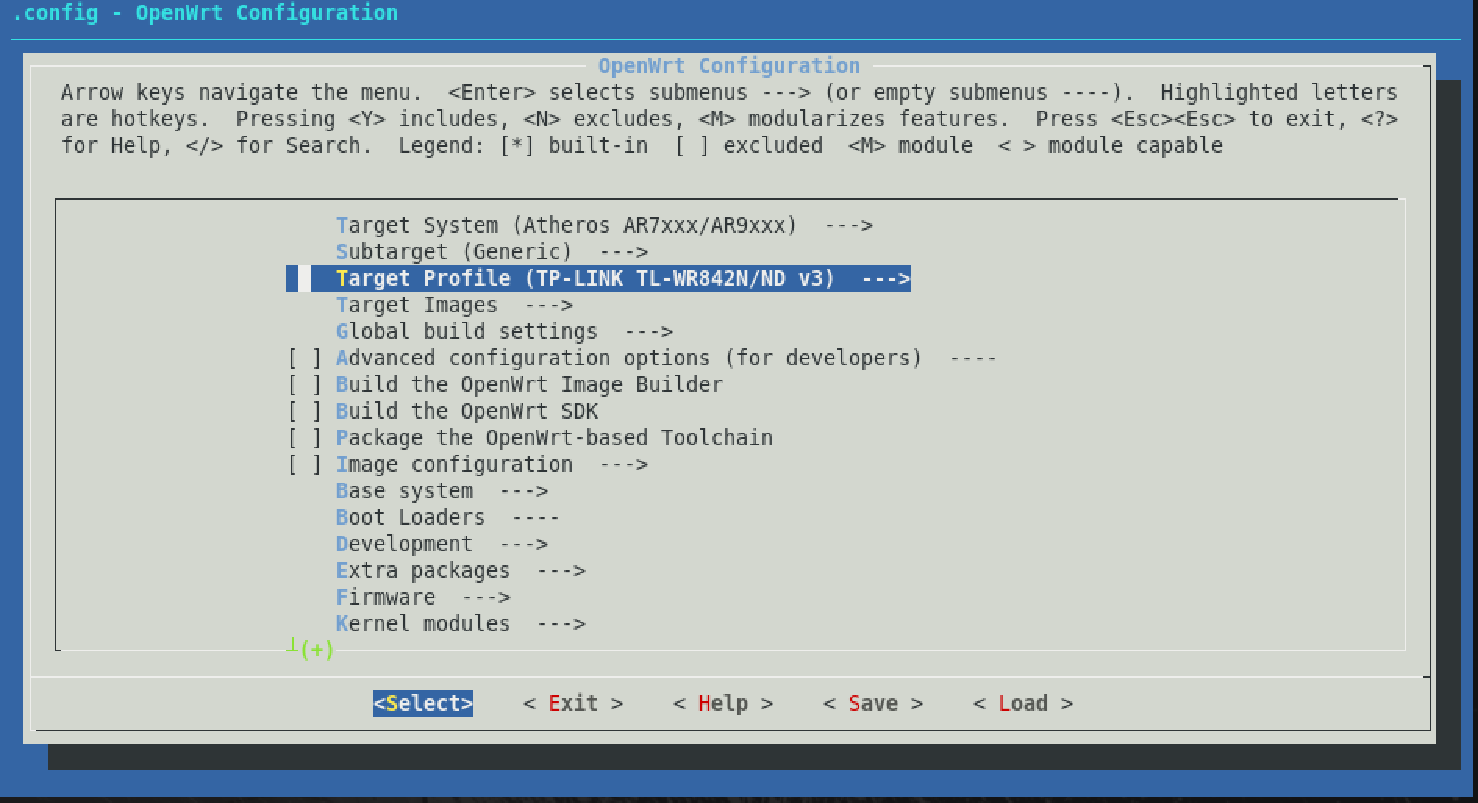
\includegraphics[scale=0.6]{figures/make_menuconfig.pdf}
    \caption{menuconfig}
    \label{fig_menuconfig}
\end{figure}
Image can be configured with three options: y, m, n which are represented as follows:
\begin{itemize}
\item pressing {\tt y} sets the {\tt <*>} built-in label\\
This package will be compiled and included in the firmware image file.
\item pressing {\tt m} sets the {\tt <M>} package label\\
This package will be compiled, but not included in the firmware image file. (E.g. to be installed with opkg after flashing the firmware image file to the device.)
\item pressing {\tt n} sets the {\tt < >} excluded label\\
The source code will not be processed.
\end{itemize}
Target system is selected from the extensive list of supported platforms, with the numerous target profiles – ranging from specific devices to generic profiles, all depending on the particular device at hand.
In our case, we should browse the {\tt Target Profile} selection and find our targeted device (TP-LINK TL-WR842N/ND v3).

Package selection has the option of either 'selecting all packages', which might be un-practical in certain situations, or relying on the default set of packages will be adequate or make an individual selection.
It is here worth mentioning that some package combinations might break the build process, so it can take some experimentation before the expected result is reached.
Added to this, the OpenWrt developers are themselves only maintaining a smaller set of packages – which include all default packages – but, the feeds-script makes it very simple to handle a locally maintained set of packages and integrate them in the build-process.

The final step before the process of compiling the intended image would be to exit the menuconfig tool – this also includes the option to save a specific configuration or load an already existing, and pre-configured, version.
Exit the UI, and choose to save the settings.
When we save our configuration, the file {\tt .config} will be created in the buildroot directory according to desired configuration \cite{build_owrt}.



\subsection{Building Single Packages}

When developing or packaging software for OpenWrt, it is convenient to be able to build only the package in question (e.g. with package cups):
\begin{lstlisting}[columns=fixed,basicstyle=\ttfamily\footnotesize,tabsize=4,backgroundcolor=\color{yellow!10}]
$ make package/cups/compile V=s
\end{lstlisting}
For a rebuild run:
\begin{lstlisting}[columns=fixed,basicstyle=\ttfamily\footnotesize,tabsize=4,backgroundcolor=\color{yellow!10}]
$ make package/cups/{clean,compile,install} V=s
\end{lstlisting}
It doesn't matter what {\it feed} the package is located in, this same syntax works for any available package.

If for some reason the build fails, the easiest way to spot the error is to do:
\begin{lstlisting}[columns=fixed,basicstyle=\ttfamily\footnotesize,tabsize=4,backgroundcolor=\color{yellow!10}]
$ make package/cups/{clean,compile,install} V=s 2>&1 | \
    tee build.log | grep -i error
\end{lstlisting}
This pipeline shown invocates the rebuild of the package forwarding the ouput to {\tt build.log} file with {\tt tee}, looking for case insensitive string 'error' with {\tt grep}.
Complete guide can be found on OpenWrt Wiki\footnote{https://wiki.openwrt.org/doc/howto/build}.
